
\todo[inline]{1. all of my commentary on performance improvement for the
sfcompo test set is outlined to go into the future work section. or should it
go here?  2. also, there may be some useful information from the model
generalization or rxtr type prior knowledge sections that could be useful here
for more in depth discussion. 3. this ended up really motivating the use of
relative error versus absolute (really, both) so it could maybe go first, then
the random error results section could go second using the relative error
plots?}

The testing described in Section \ref{sec:randerr} describes the process of
evaluating the methodology with test cases drawn from the training database.
It is also helpful to test the methodology against real assays of \gls{SNF}.
The \gls{SFCOMPO} database was created to allow access to these sorts of
measurements linked to the reactor operation parameters being predicted in this
work. \cite{sfcompo}. The only parameter not part of the \gls{SFCOMPO} database
is the time since irradiation, so that is not predicted here. 

\begin{figure}[!htb]
  \centering
  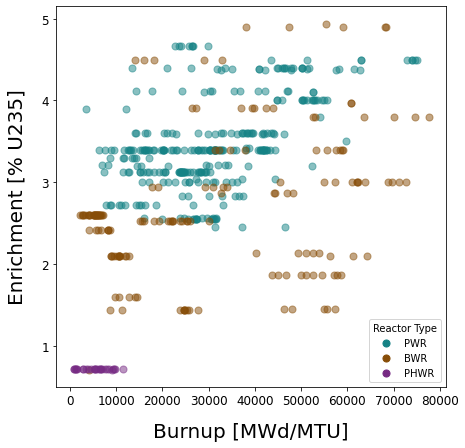
\includegraphics[width=0.7\textwidth]{./chapters/exp1/sfcompo_scatter_viz.png}
  \caption{Scatter plot showing the range of reactor operation parameters in 
           the \gls{SFCOMPO} testing set that are being predicted.}
  \label{fig:sfcoscatter}
  \todo[inline]{maybe show comparison against training E v B scatter plot}
\end{figure}

There are 505 test cases that are able to be compared against the training
database.  The number of each reactor type is as follows: 312 \gls{PWR}s, 165
\gls{BWR}s, and 28 \gls{PHWR}s. The space of enrichment and burnup values is
visualized in Figure \ref{fig:sfcoscatter}. These are sufficiently represented
in the training set design, as pictured in Figure \ref{fig:trainhist}, although
the proportions of \gls{PWR} and \gls{BWR} are approximately opposite to the
training set. The assays in \gls{SFCOMPO} are presented as nuclide
concentrations with the units \textit{milligrams per grams of initial uranium},
or $mg/gU_i$. The training set of nuclide measurements in \textit{grams} is
converted to these concentration units prior to prediction is converted to
these concentration units prior to prediction. 

There is one main issue with using \gls{SFCOMPO} as a testing set: missing
nuclide measurements.  The feature set of 29 nuclides in Table
\ref{tbl:nucmass} was chosen based on the frequency of these measurements being
present in the database at an arbitrary level of 100 measurements. This
happened before filtering, so there are some nuclide measurements present at
under 100 counts.  Each nuclide's frequency in \gls{SFCOMPO} is listed in Table
\ref{tbl:missing}.  While every assay contains several plutonium measurements
and most contain uranium measurements as well, the remaining nuclides are
present at a much lower rate. 

\begin{table}[!htb]
  \centering
  \begin{tabular}{>{\raggedleft}m{0.6in}
                                m{0.4in}
                  >{\raggedleft}m{0.6in}
                                m{0.4in}
                  >{\raggedleft}m{0.6in}
                                m{0.4in}}
    \toprule
    \rowcolor[gray]{0.88} am241  & 237 & nd145 & 162 & sm147 & 97  \\  
    \rowcolor[gray]{0.95} am242m & 110 & nd146 & 139 & sm149 & 97  \\ 
    \rowcolor[gray]{0.88} am243  & 203 & nd148 & 275 & sm150 & 97  \\ 
    \rowcolor[gray]{0.95} cm242  & 214 & nd150 & 121 & sm151 & 97  \\ 
    \rowcolor[gray]{0.88} cm244  & 269 & np237 & 155 & sm152 & 97  \\ 
    \rowcolor[gray]{0.95} cs134  & 113 & pu238 & 369 & u234  & 355 \\ 
    \rowcolor[gray]{0.88} cs137  & 185 & pu239 & 505 & u235  & 479 \\ 
    \rowcolor[gray]{0.95} eu154  & 100 & pu240 & 505 & u236  & 462 \\ 
    \rowcolor[gray]{0.88} nd143  & 162 & pu241 & 504 & u238  & 433 \\ 
    \rowcolor[gray]{0.95} nd144  & 113 & pu242 & 505 &       &     \\ \bottomrule
  \end{tabular}
  \caption{Number of assays each nuclide is measured for in the \gls{SFCOMPO}
           database.}
  \label{tbl:missing}
\end{table}

Although some algorithms in theory can handle null values in the training
stage, scikit-learn does not currently include this capability. The \gls{MLL}
method is designed to handle null values, however. This is done by converting
them to zero and filtering out all zero-valued nuclides during the likelihood
calculations. But there is a technique more commonly applied than converting
missing values to zero: imputation. This involves taking the mean or median of
the existing features and applying that value to the assays in which it is
missing.  The remainder of this section dicusses using the three algorithms to
predict the \gls{SFCOMPO} test cases where the nulls are both converted to zero
and imputed using the mean.  \todo[inline]{is converting to zero technically
imputation as well?}

\subsubsection{Reactor Type Classification}

Table \ref{tbl:sfcorxtr} presents two metrics for the two missing value
techniques: the accuracy and balanced accuracy scores. The accuracy scores for
both the imputed nulls and zero-nulls test sets are mostly under 0.62, which is
the fraction of \gls{PWR} entries.  Therefore, a classifier could predict
\gls{PWR} every time and do better than these accuracy scores.  For the
zero-nulls test set predictions using \gls{MLL}, however, the accuracy of 0.72
does exceed the "majority guess" accuracy of 0.62.  Since \gls{MLL}
calculations filter out null values, it is expected that the scores will be
higher for all prediction categories where \gls{MLL} is being used with the
zero-nulls test set. This expected \gls{MLL} performance also holds true when
looking at the balanced accuracy score.  A balanced accuracy score of 0 denotes
random guessing, but it can also be negative if the classifications are worse
than random guessing. The balanced accuracy of 0.63 for the zero-nulls case is
a promising result. The balanced accuracies of \textit{k}-nearest neighbors and
decision trees are all quite low. Also, the higher accuracies correspond to lower
balanced accuracies, and vice versa. Therefore, further investigation is
necessary.

\begin{table}[!htb]
  \centering
  \begin{tabular}{@{}m{1.5in}llllll@{}}
    \toprule
    & \multicolumn{3}{m{2in}}{Accuracy Scores} 
    & \multicolumn{3}{l}{Balanced Accuracy Scores} \\ 
    \toprule
    Null Handling    & kNN   & DTree  & MLL   & kNN   & DTree  & MLL    \\ \midrule
    Imputed Nulls    & 0.52  & 0.60   & 0.39  & 0.09  & 0.12   & -0.01  \\
    Zero-value Nulls & 0.45  & 0.42   & 0.72  & 0.21  & 0.30   & 0.63   \\ \bottomrule
    \end{tabular}
  \caption{Accuracy and balanced accuracy scores for reactor type prediction 
           of the \gls{SFCOMPO} test cases.}
  \label{tbl:sfcorxtr}
\end{table}

\begin{figure}[!htb]
  \centering
  \begin{subfigure}[b]{\textwidth}
    \centering
    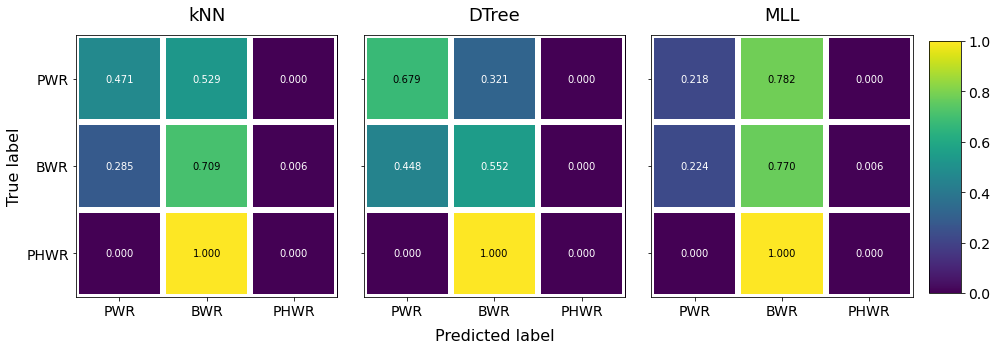
\includegraphics[width=\textwidth]{./chapters/exp1/confusion_matrix_sfco_impnull.png}
    \caption{Confusion matrices for mean-imputed null values.}
    \label{fig:cmimp}
  \end{subfigure}
  \vskip\baselineskip
  \begin{subfigure}[b]{\textwidth}
    \centering
    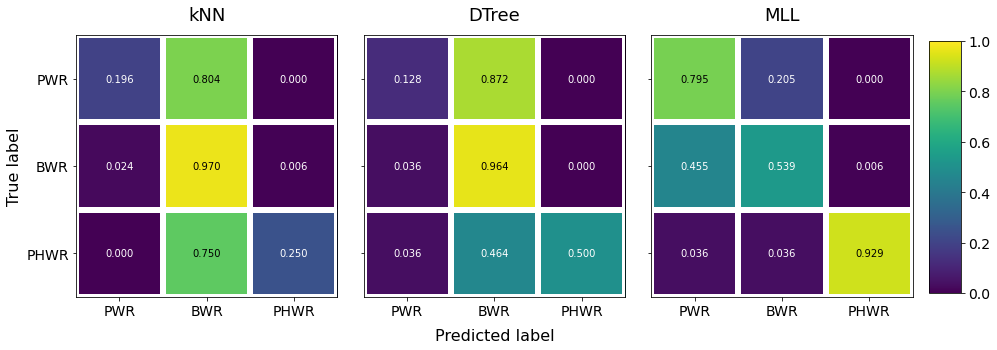
\includegraphics[width=\textwidth]{./chapters/exp1/confusion_matrix_sfco_0null.png}
    \caption{Confusion matrices for zero-replaced null values.}
    \label{fig:cm0}
  \end{subfigure}
  \caption{Confusion matrices of reactor type prediction for each algorithm 
           using two missing entry techniques: imputation with mean values 
           and replacement with zero.}
  \label{fig:cm}
\end{figure}

Figure \ref{fig:cm} allows for a deeper look into what is happening with the
reactor type predictions for both of the \gls{SFCOMPO} test sets.  The matrices
from using mean-imputed null values are in Figure \ref{fig:cmimp} and the
matrices from using zero-filled null values are in Figure \ref{fig:cm0}.  The
scikit-learn algorithms have a higher accuracy for the imputed null values test
set than their zero-null values counterparts, but the balanced accuracies
follow the opposite direction. For \textit{k}-nearest neighbors, imputed nulls
cause more than half of the \gls{PWR}s and all of the \gls{PHWR}s to be
misclassified as \gls{BWR}s. Additionally, 28.5\% \gls{BWR}s are misclassified
as \gls{PWR}s.  For the zero-nulls test set, there is a much larger correct
\gls{BWR} classification percentage, but also a much larger \gls{PWR}
misclassification percentage. The \gls{PHWR} true positive percentage increases
from 0 to 25\%. \Gls{BWR} (32\% of test cases) and \gls{PHWR} (5.5\% of test
cases) are the two minority classes in the database.  Because they both have
higher true positive fractions but there were overall fewer correct predictions
(from a much higher \gls{PWR} misclassification) from the imputed nulls to the
zero-nulls, the accuracy went down but the balanced accuracy went up.

Decision trees follows a similar pattern the the \textit{k}-nearest neighbors
example.  The \gls{PWR} misclassification increases from the imputed nulls to
the zero-nulls test set in a similar manner, although the original \gls{PWR}
true positive fraction is higher (leading to a higher accuracy for the imputed
nulls case).  As before, the \gls{BWR} correct classification increases
drastically from the imputed nulls to zero-nulls case.  Additionally, the
\gls{PHWR} classifiction improvement from imputed nulls to zero-nulls is better
for decision trees than for \textit{k}-nearest neighbors.  Therefore, again,
the accuracy decreased and the balanced accuracy increased. The larger
improvement for the minority classes has led to the larger balanced accuracy
improvement for decision trees.

In Figure \ref{fig:cm}, the confusion matrices for the \gls{MLL} calculations
tell a very different story than those for the scikit-learn algorithms.  The
only similarity is that using imputed nulls causes all \gls{PHWR}s to be
classified as \gls{BWR}s. \gls{PWR}s are misclassified as \gls{BWR}s at 78.2\%,
and \gls{BWR}s are misclassified as \gls{PWR}s at 22.4\%. For the zero-nulls
test set, \gls{PHWR}s and \gls{PWR}s true positive percentages sharply improve
to 92.9\% and 79.5\%, respectively.  The true positive rate for \gls{BWR}s,
however, decreases from 77.0\% to 53.9\%. This is the opposite trend from both
of the scikit-learn algorithms.  Despite the misclassification increase for
\gls{BWR}s, both the accuracy score and balanced accuracy score increase for
\gls{MLL} calculations when moving from using imputed null values to zero-null
values in the test set. The improvement in \gls{MLL} classification is likely
because the imputed nulls test set hides information rather than removing it
from consideration, which is what the zero-nulls test set does. 

All three algorithms using both test sets tend towards misclassifying
\gls{PHWR}s as \gls{BWR}s (except for \gls{MLL} calculations using zero-null
missing values).  This is likely because \gls{BWR}s comprise the majority of
the training set (72\%), and no matter how the missing measurements are handled
there may be too little information to predict these well with most algorithms.
For the two scikit-learn algorithms, the zero-nulls test set predicts
\gls{BWR}s the majority of the time (despite there being 50\% correct
\gls{PHWR} prediction for decision trees). This also is likely from \gls{BWR}
being the training set majority class, so with many nuclides measuring at zero,
there are likely to be few good matches, and the majority class becomes the
most likely prediction. This explanation is possibly applicable to the imputed
nulls test set as well, but the behavior pattern is less clear because the
imputed nulls give more information for these algorithms than zero-value nulls
(since the zero-values cannot be removed from consideration), so a larger
proportion of \gls{PWR}s are being predicted properly.  \todo[inline]{look up
paper that uses only U/Pu to predict, because that would be the only way these
505 cases would be able to be predicted without having so much missing
information. MLL essentially does this for 0 null case which is why it does
better than the rest}

\subsubsection{Regression Cases}

Next, the prediction of \gls{SFCOMPO} test samples for the regression cases
will be discussed. There is no time since irradiation value in the database, so
only burnup and \gls{U235} enrichment are discussed here.  While the mean and
median errors for burnup and enrichment prediction are listed in Tables
\ref{tbl:sfcoburn} and \ref{tbl:sfcoenri}, respectively, there are also box
plots inlcuded for both absolute and relative errors in Figures
\ref{fig:sfcoburn} and \ref{fig:sfcoenri}, respectively.  Box plots were chosen
since they can provide a larger amount of information than just a mean or
median value.  The white triangles represent the mean error, and the white line
in notched box is the median error. The box itself is the 25\% (Q1) and 75\%
(Q3) quartiles at the bottom and top, respectively. The error bars or whiskers
are meant to represent the spread of all errors minus the outliers.  The bottom
whisker reaches to $Q1 - 1.5*(Q3-Q1)$ and the top whisker reaches to $Q3 +
1.5*(Q3-Q1)$. Any values outside of this range are considered outliers.
\cite{matplotlib}

\noindent \textbf{Burnup}

The expected results that \gls{MLL} will perform better with the zero-nulls
test set also holds true for the regression cases, as shown in Table
\ref{tbl:sfcoburn}.  While the scikit-learn algorithms have a moderate increase
in both the mean and median burnup errors from the imputed nulls to the
zero-nulls, the \gls{MLL} calculations have an order of magnitude decrease in
error when moving in that same direction.  Seeing this trend between Figures
\ref{fig:burnimp} and \ref{fig:burn0} is a little difficult due to the
different ranges on the \textit{y}-axes, but the drastic improvement in
\gls{MLL} burnup error from the imputed nulls in Figure \ref{fig:burnimp} to
the zero-nulls in Figure \ref{fig:burn0} is still visually clear. In the latter
figure, there is one outlier for \textit{k}-nearest neighbors and 39 for
\gls{MLL} calculations.

\begin{table}[!htb]
  \centering
  \begin{tabular}{@{}m{1.5in}llllll@{}}
    \toprule
                     & \multicolumn{3}{m{2in}}{Mean Errors [GWd/MTU]} & \multicolumn{3}{c}{Median Errors [GWd/MTU]} \\ \toprule
    Null Handling    & kNN           & DTree         & MLL           & kNN            & DTree          & MLL    \\ \midrule
    Imputed Nulls    & 9.43          & 10.89         & 13.17         & 7.26           & 8.28           & 10.84  \\
    Zero-value Nulls & 14.88         & 15.18         & 3.53          & 11.47          & 8.79           & 1.70   \\ \bottomrule
  \end{tabular}
  \caption{Mean and median errors for burnup prediction of the \gls{SFCOMPO} 
           test cases.}
  \label{tbl:sfcoburn}
\end{table}

Although the mean and median errors are contained in the range of $1-15
GWd/MTU$, the large spread in burnup errors in Figures \ref{fig:burnimp} and
\ref{fig:burn0} for all three algorithms was broad enough to warrant an
investigation into the range of relative errors, expressed as percent errors in
Figures \ref{fig:burnimppct} and \ref{fig:burn0pct}.  In Figure
\ref{fig:burnimppct} there are 75, 72, and 73 outliers (all around 15\% of the
test database) for the \textit{k}-nearest neighbors, decision trees, and
\gls{MLL} calculations, respectively.  In Figure \ref{fig:burn0pct} there are
45 outliers for the \gls{MLL} calculations.

\begin{figure}[!htb]
  \centering
  \begin{subfigure}[b]{0.49\textwidth}
    \centering
    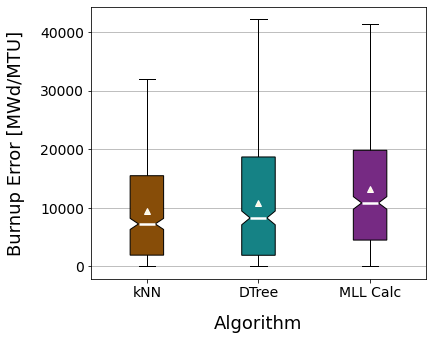
\includegraphics[width=\textwidth]{./chapters/exp1/sfcompo_boxplots_impnull_burn.png}
    \caption{Box plots of burnup errors using mean-imputed null values.}
    \label{fig:burnimp}
  \end{subfigure}
  \hfill
  \begin{subfigure}[b]{0.49\textwidth}
    \centering
    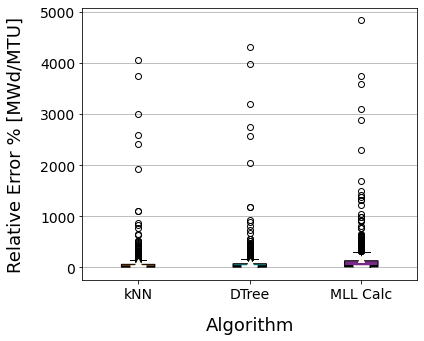
\includegraphics[width=\textwidth]{./chapters/exp1/sfcompo_boxplots_impnull_pcterr_burn.png}
    \caption{Box plots of burnup percentage errors using mean-imputed null values.}
    \label{fig:burnimppct}
  \end{subfigure}
  \vskip\baselineskip
  \begin{subfigure}[b]{0.49\textwidth}
    \centering
    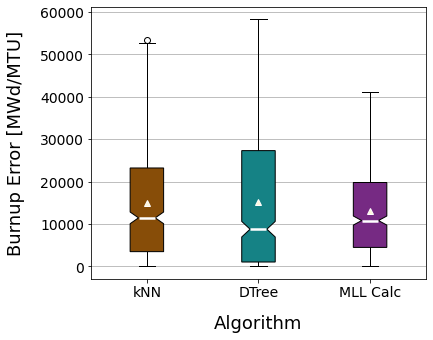
\includegraphics[width=\textwidth]{./chapters/exp1/sfcompo_boxplots_0null_burn.png}
    \caption{Box plots of burnup errors using zero-replaced null values.}
    \label{fig:burn0}
  \end{subfigure}
  \hfill
  \begin{subfigure}[b]{0.49\textwidth}
    \centering
    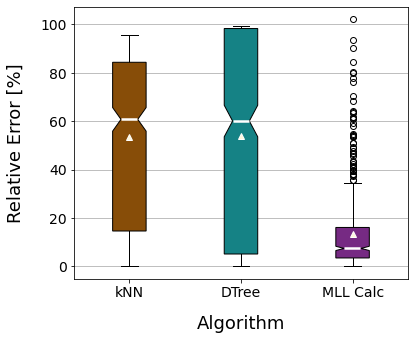
\includegraphics[width=\textwidth]{./chapters/exp1/sfcompo_boxplots_0null_pcterr_burn.png}
    \caption{Box plots of burnup percentage errors using zero-replaced null values.}
    \label{fig:burn0pct}
  \end{subfigure}
  \caption{Box plots of burnup prediction errors and percentage errors for each 
           algorithm using two missing entry techniques: imputation with mean 
           values and replacement with zero.}
  \label{fig:sfcoburn}
\end{figure}

The ranges seen for the imputed nulls test set in Figure \ref{fig:burnimppct}
are as large as they are from low burnups ($< 10 GWd/MTU$) being far
overpredicted, since a small number in the denominator will yield a high
percentage error. A large subset of the low burnup cases are \gls{PHWR}s.
Their burnups are also unlikely to be predicted well because of the inability
of \gls{PHWR} reactors to be represented accurately with this methodology.
Removing the \gls{PHWR} reactors from the results removes all outliers with
percentage errors larger than 1750\%. That is still a very high relative error,
but there are other low burnup cases in the database.  Removing \gls{PHWR}s
does not significantly alter the zero-nulls results in Figure
\ref{fig:burn0pct}.

The range of percentage errors for the zero-nulls test set in Figure
\ref{fig:burn0pct} tells a different story. There is only one case (an
\gls{MLL} outlier) that is above 100\% error.  While the absolute errors for
the scikit-learn algorithms in Figure \ref{fig:burn0} span a larger range than
their counterparts in Figure \ref{fig:burnimp}, their relative errors remain
within $0-100\%$. The only case that predicts the burnup well is the \gls{MLL}
method with the zero-null missing values treatment of the \gls{SFCOMPO} test
set, but about 8\% of the test cases are outliers.  If the best-case median
error of $1.7 GWd/MTU$ in Table \ref{tbl:sfcoburn} were to also correspond to a
lower relative error, then that would be an acceptable result.  However, while
the \gls{MLL} calculations have a percentage error below 20\% at the 75\%
quartile, the non-outlier data reaches almost 40\% and the 8\% of the data
reaches 100\%.

Overall, the absolute errors in Table \ref{tbl:sfcoburn} tell a much more
encouraging story than the box plots in Figure \ref{fig:sfcoburn}, so
investigating beyond the mean and median absolute errors was necessary to show
the real picture of this unique testing scenario. 

\noindent \textbf{\gls{U235} Enrichment}

For both reactor type classification and burnup regressoion, the zero-nulls
test set predicted by \gls{MLL} calculations far outperform all other
algorithm/test set scenarios. However, the enrichment regression results break
this trend.  Table \ref{fig:sfcoenri} shows that decision trees outperform the
other methods, and furthermore, there isn't a large difference in performance
between the two test sets, expecially seeing that the median absolute error is
the same for both test sets.  The other two algorithms follow their previous
behavior: moving from imputed nulls to zero-nulls, \textit{k}-nearest neighbors
has worse performance and \gls{MLL} calculations has better performance.

\begin{table}[!htb]
  \centering
  \begin{tabular}{@{}m{1.5in}llllll@{}}
    \toprule
                     & \multicolumn{3}{m{2in}}{Mean Errors [\% U235]} & \multicolumn{3}{l}{Median Errors [\% U235]} \\ \toprule
    Null Handling    & kNN           & DTree          & MLL          & kNN            & DTree          & MLL    \\ \midrule
    Imputed Nulls    & 0.72          & 0.31           & 1.25         & 0.50           & 0.22           & 1.13   \\
    Zero-value Nulls & 1.67          & 0.36           & 0.49         & 2.02           & 0.22           & 0.35   \\ \bottomrule
  \end{tabular}
  \caption{Mean and median errors for enrichment prediction of the \gls{SFCOMPO} 
           test cases.}
  \label{tbl:sfcoenri}
\end{table}

The mean and median absolute errors are also visible with more statistical
information in the box plots in Figure \ref{fig:sfcoenri}. The outliers for
decision trees and \gls{MLL} calculations are 30 and 16 for the imputed nulls
in Figure \ref{fig:enriimp}, respectively. So although decision trees provides
a typically low absolute error, the outliers reach nearly as far as the spread
of \textit{k}-nearest neighbors. The number of outliers for the zero-nulls
results in Figure \ref{fig:enri0} are 45 and 16 for decision trees and
\gls{MLL} calculations, respectively.  The spread of the outliers for these
algorithms is similar to the previous figure, but \textit{k}-nearest neighbors
has a larger spread of absolute error.

\begin{figure}[!htb]
  \centering
  \begin{subfigure}[b]{0.49\textwidth}
    \centering
    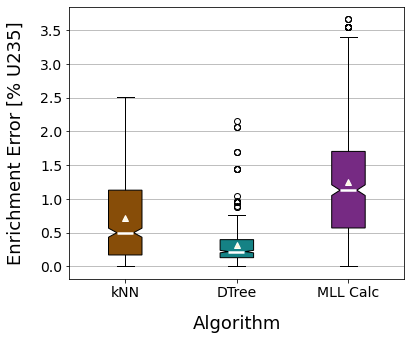
\includegraphics[width=\textwidth]{./chapters/exp1/sfcompo_boxplots_impnull_enri.png}
    \caption{Box plots of enrichment errors using mean-imputed null values.}
    \label{fig:enriimp}
  \end{subfigure}
  \hfill
  \begin{subfigure}[b]{0.49\textwidth}
    \centering
    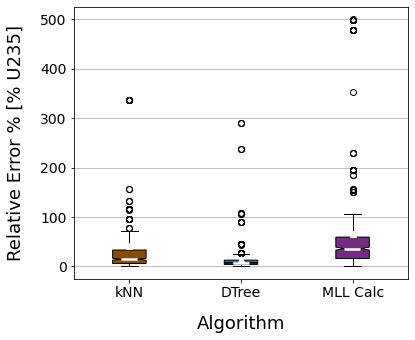
\includegraphics[width=\textwidth]{./chapters/exp1/sfcompo_boxplots_impnull_pcterr_enri.png}
    \caption{Box plots of enrichment percentage errors using mean-imputed null values.}
    \label{fig:enriimppct}
  \end{subfigure}
  \vskip\baselineskip
  \begin{subfigure}[b]{0.49\textwidth}
    \centering
    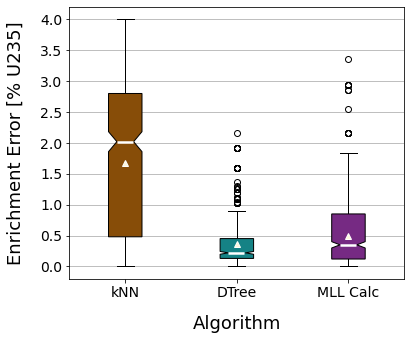
\includegraphics[width=\textwidth]{./chapters/exp1/sfcompo_boxplots_0null_enri.png}
    \caption{Box plots of enrichment errors using zero-replaced null values.}
    \label{fig:enri0}
  \end{subfigure}
  \hfill
  \begin{subfigure}[b]{0.49\textwidth}
    \centering
    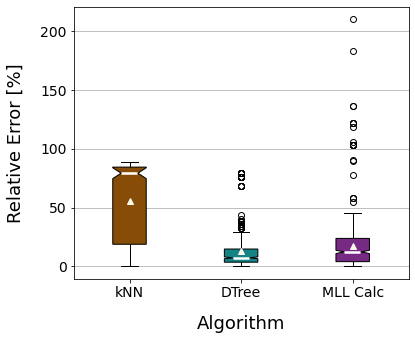
\includegraphics[width=\textwidth]{./chapters/exp1/sfcompo_boxplots_0null_pcterr_enri.png}
    \caption{Box plots of enrichment percentage errors using zero-replaced null values.}
    \label{fig:enri0pct}
  \end{subfigure}
  \caption{Box plots of enrichment prediction errors and percentage errors for 
           each algorithm using two missing entry techniques: imputation with 
           mean values and replacement with zero.}
  \label{fig:sfcoenri}
\end{figure}

Again, a look at the relative errors gives a different sense of these results.
Figures \ref{fig:enriimppct} and \ref{fig:enri0pct} present the percent error
statistics for the imputed nulls and zero-nulls test sets, respectively.  In
Figure \ref{fig:enriimppct} there are 57, 39, and 49 outliers for the
\textit{k}-nearest neighbors, decision trees, and \gls{MLL} calculations,
respectively.  In Figure \ref{fig:enri0pct} there are 44 and 23 outliers for
the decision trees and \gls{MLL} calculations, respectively.

As with the burnup regression, the high percentage errors are caused by a large
overprediction of enrichments that are of low value. All of the \gls{PHWR}s fit
into this category, and removing them from the results removes the outliers
with the highest errors from the imputed nulls results in Figure
\ref{fig:enriimppct}, leaving a maximum of 250\% enrichment error. This is
still a high maximum error because there are other low enrichments not
belonging to the \gls{PHWR} class that remain overpredicted.  As with the
burnup, removing \gls{PHWR}s does not significantly alter the zero-nulls
results in Figure \ref{fig:enri0pct}.

Unlike the case with burnup, the decision trees algorithm gives a better
performance that is null handling-independent than the other algorithm/test set
scenarios. Although there was a slightly worse mean absolute error for the
zero-nulls test set (the median absolute error was the same), the relative
error remains below 100\% for all outliers, as seen in Figure
\ref{fig:enri0pct}.  This makes the decision trees algorithm with the
zero-nulls test set the best performing case for enrichment regression.

It is again true that investigating relative error statistics alongside
absolute error statistics provides a fuller picture of the regression of the
\gls{SFCOMPO} database entries.  It is an unexpected result to have either one
of the scikit algorithms outperform \gls{MLL} calculations for the zero-nulls
test set, since they tended to have lower errors using the imputed nulls test
set. 

